Parmi les habitants âgés d'au moins 15 ans vivant en France, on compte :

\begin{itemize}[label=\textbullet~]
	\item $21~\%$ de personnes de 15 à 29 ans;
	\item $46~\%$ de personnes de 30 à 59 ans;
	\item $33~\%$ de personnes d'au moins 60 ans.
\end{itemize}

On s'intéresse à l'utilisation d'un réseau social par les habitants âgés d'au moins 15 ans vivant en France. On a ainsi pu observer que :

\begin{itemize}[label=\textbullet~]
	\item $70~\%$ des personnes de 15 à 29 ans ont déjà publié sur ce réseau social;
	\item $46~\%$ des personnes de 30 à 59 ans ont déjà publié sur ce réseau social;
	\item $15~\%$ des personnes d'au moins 60 ans ont déjà publié sur ce réseau social.
\end{itemize}

On interroge une personne âgée d'au moins 15 ans vivant en France et on lui demande si elle a déjà publié sur ce réseau social.

On note :

\begin{itemize}[label=\textbullet~]
	\item $J$ l'événement : \og la personne interrogée a entre 15 et 29 ans \fg{};
	\item $M$ l'événement : \og la personne interrogée a entre 30 et 59 ans \fg{};
	\item $S$ l'événement : \og la personne interrogée a au moins 60 ans \fg{};
	\item $R$ l'événement: \og la personne interrogée a déjà publié sur ce réseau social \fg{}.
\end{itemize}

On note $\overline{R}$ l'événement contraire de l'événement $R$.

Dans tout l'exercice, les valeurs approchées seront arrondies au millième.

\subsection*{Partie A}
\begin{enumerate}
	\item Recopier et compléter l'arbre de probabilité.

	
	\begin{center}
		
		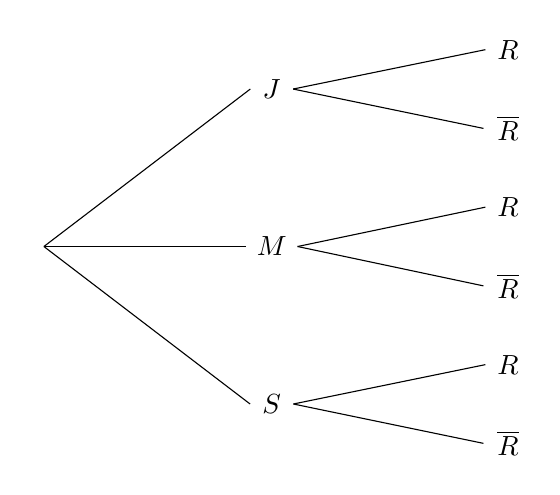
\begin{tikzpicture}[xscale=1,yscale=1]
			
			\tikzstyle{noeud}=[fill=white,circle,inner sep=2pt]
			\tikzstyle{feuille}=[fill=white,circle,inner sep=2pt]
			\tikzstyle{etiquette}=[midway,fill=white, inner xsep=3pt, inner ysep=1.5pt]
			
			\def\DistanceInterNiveaux{3}
			\def\DistanceInterFeuilles{1}
			
			\def\NiveauA{(0)*\DistanceInterNiveaux}
			\def\NiveauB{(1)*\DistanceInterNiveaux}
			\def\NiveauC{(2)*\DistanceInterNiveaux}
			\def\InterFeuilles{(-1)*\DistanceInterFeuilles}
			
			\node[noeud] (R) at ({\NiveauA},{(2.5)*\InterFeuilles}) {$$};
			\node[noeud] (Ra) at ({\NiveauB},{(0.5)*\InterFeuilles}) {$J$};
			\node[feuille] (Raa) at ({\NiveauC},{(0)*\InterFeuilles}) {$R$};
			\node[feuille] (Rab) at ({\NiveauC},{(1)*\InterFeuilles}) {$\overline{R}$};
			\node[noeud] (Rb) at ({\NiveauB},{(2.5)*\InterFeuilles}) {$M$};
			\node[feuille] (Rba) at ({\NiveauC},{(2)*\InterFeuilles}) {$R$};
			\node[feuille] (Rbb) at ({\NiveauC},{(3)*\InterFeuilles}) {$\overline{R}$};
			\node[noeud] (Rc) at ({\NiveauB},{(4.5)*\InterFeuilles}) {$S$};
			\node[feuille] (Rca) at ({\NiveauC},{(4)*\InterFeuilles}) {$R$};
			\node[feuille] (Rcb) at ({\NiveauC},{(5)*\InterFeuilles}) {$\overline{R}$};
			
			\draw (R.east)--(Ra.west);
			\draw (Ra.east)--(Raa.west);
			\draw (Ra.east)--(Rab.west);
			\draw (R.east)--(Rb.west);
			\draw (Rb.east)--(Rba.west);
			\draw (Rb.east)--(Rbb.west);
			\draw (R.east)--(Rc.west);
			\draw (Rc.east)--(Rca.west);
			\draw (Rc.east)--(Rcb.west);
		\end{tikzpicture}
	\end{center}
	


	\item Déterminer $P(M \cap R)$.

	Interpréter le résultat dans le contexte de l'exercice.

	\item On interroge au hasard une personne âgée d'au moins 15 ans vivant en France.

	\begin{enumerate}
		\item Calculer la probabilité qu'elle ait déjà publié sur ce réseau social.

		\item On sait que cette personne a déjà publié sur ce réseau social.

		Déterminer la probabilité qu'elle ait au moins 60 ans.
	\end{enumerate}
\end{enumerate}

\subsection*{Partie B}
Au cours d'un sondage, on interroge successivement, au hasard et de manière indépendante, 100 personnes âgées d'au moins 15 ans vivant en France et on leur demande si elles ont déjà publié sur ce réseau social.

La population du pays est suffisamment grande pour qu'on assimile le choix des personnes sondées à des tirages successifs avec remise.

On note $X$ la variable aléatoire qui donne le nombre de personnes ayant déjà publié sur ce réseau social parmi ces 100 personnes interrogées.

Dans cette partie, on admet que la probabilité qu'une personne âgée d'au moins 15 ans vivant en France ait déjà publié sur ce réseau social est 0,41.

\begin{enumerate}
	\item On admet que la variable aléatoire $X$ suit une loi binomiale.

	Donner ses paramètres.

	\item Calculer la probabilité qu'au moins la moitié des 100 personnes interrogées ait déjà publié sur ce réseau social.

	\item Déterminer l'espérance de la variable aléatoire $X$ et interpréter le résultat dans le contexte de l'exercice.
\end{enumerate}

\subsection*{Partie C}
On effectue le sondage décrit dans la \textbf{partie B} dans 150 villes françaises en respectant les mêmes conditions.

On note $X_{1}$\,, $X_{2}$\,, \ldots\,, $X_{150}$ les variables aléatoires donnant le nombre de personnes ayant déjà publié sur ce réseau social parmi les 100 personnes interrogées dans chacune des 150 villes.

On considère $Y$ la variable aléatoire définie par :
\[Y=\dfrac{X_{1}+X_{2}+\cdots+X_{150}}{150}\]

Démontrer que la probabilité que la variable aléatoire $Y$ soit strictement comprise entre 37 et 45 est strictement supérieure à $98~\%$.
